% !TEX TS-program = pdflatex
\documentclass[a4paper]{article} 
\usepackage{listings}
\usepackage{hyperref}
\usepackage{fancyhdr}
\usepackage{graphicx}
\usepackage[table]{xcolor}
\usepackage{color}
\usepackage{tabularx}
\usepackage[top=3.5cm, bottom=3.5cm, left=2.5cm, right=4.5cm]{geometry} 
\usepackage{indentfirst}

% Margin notes: 
\newcommand{\mnote}[1]{\marginpar{\small{\textcolor{red}{\texttt{#1}}}}}

% Start the document here:
\begin{document}
	
% Font configuration:
\fontfamily{cmr}
\fontsize{12}{15}
\selectfont

% Headers and footers:
\pagestyle{fancy}
\fancyhead[L]{STIX Specifications}
\fancyhead[R]{Version 0.1}
\fancyfoot[C]{\thepage}
\renewcommand{\headrulewidth}{0.4pt}
\renewcommand{\footrulewidth}{0.4pt}

% Code syntax highlighting:
\definecolor{light-gray}{gray}{0.92}
\lstset{
	frame			= single, 
	backgroundcolor	= \color{light-gray}, 
	tabsize			= 2, 
	basicstyle		= \ttfamily\small,
	morecomment		= [s]{!--}{--},
	keywordstyle	= \textbf,
	commentstyle	= \textit,
	stringstyle		= \textit,
	breakautoindent	= true,
	breakindent		= 2em,
	breaklines		= true,
	postbreak		= ,
	%prebreak		= \raisebox{-.8ex}[0ex][0ex]{\ensuremath{\lrcorner}},
	prebreak		= \raisebox{-.8ex}[0ex][0ex]{\Righttorque},
	showspaces		= false,
	showtabs		= false,
	showstringspaces= false,
}

% Title and abstract:
\title{\textbf{STIX Specification Document}}
\author{Giacomo Bernardi, Matt Calder, Damon Fenacci, Alex Macmillan} 
\date{\today}
\maketitle

\begin{center}
Version: \texttt{0.1} \\
Project mailing-list: \texttt{\href{mailto:stix@inf.ed.ac.uk}{stix@inf.ed.ac.uk}} \\
Project website: \texttt{\href{http://www.wimo.inf.ed.ac.uk/stix}{http://www.wimo.inf.ed.ac.uk/stix}}
\end{center}

% Abstract: I don't know why, but it HAS TO be as a single paragraph
\renewcommand*\abstractname{}
\begin{abstract}
\large\emph{
The present document provides the specifications of the STIX network management system, intending to be used as guidelines for the implementation and evaluation steps.\\
\indent We describe the basic architecture of the system, the visual paradigm used, its basic constructs and we provide suggestions about the internal mechanisms for an efficient coding and use. Finally, in the Appendix we envision three ``Use Cases'' that can be used to verify and evaluate the system.\\
\indent The specifications contained in this text are considered as a minimum set of requirements for the STIX implementation to be of practical use, further features will be introduced with future revisions of this document.
}\end{abstract}

% Table of contents:
\newpage
\renewcommand*\contentsname{Table of Contents}
\makeatletter
\renewcommand\l@section[2]{%
  \ifnum \c@tocdepth >\z@
    \addpenalty\@secpenalty
    \addvspace{1.0em \@plus\p@}%
    \setlength\@tempdima{1.5em}%
    \begingroup
      \parindent \z@ \rightskip \@pnumwidth
      \parfillskip -\@pnumwidth
      \leavevmode \bfseries
      \advance\leftskip\@tempdima
      \hskip -\leftskip
      #1\nobreak\ 
      \leaders\hbox{$\m@th\mkern \@dotsep mu\hbox{.}\mkern \@dotsep mu$}
     \hfil \nobreak\hb@xt@\@pnumwidth{\hss #2}\par
    \endgroup
  \fi}
\makeatother
\tableofcontents

% Vertical space between paragraphs:
\setlength{\parskip}{1ex plus 0.5ex minus 0.2ex}

\label{sec:terminology}
\section{Terminology}
\vspace{0.2cm}
\noindent
\begin{tabularx}{\textwidth}{| p{4cm} | X | }
	\hline 
	\cellcolor[gray]{0.9} \textbf{Term:} & \cellcolor[gray]{0.9} \textbf{Description:} \\ \hline 
	IDE 					& Integrated Development Environment \\	\hline 
	BTS 					& Base Transmitting Station, a device located on a transmitting site which is part of the service provider infrastructure \\ \hline 
	CPE 					& Customer Premises Equipment, a device housed at user’s premises that act as network endpoint \\ \hline 
	User or Administrator 	& The user of the NPMN management platform, typically the network administrator. \\ \hline
	Task 					& A basic management task, implemented in binary form and installed in the Task Library. \\ \hline 
\end{tabularx}

% Here start the real document:
\newpage
\label{sec:introduction}
\section{Introduction}
\noindent\textbf{Project scope:}

The aim of the STIX project is to design, implement and evaluate a framework for network management of Broadband Wireless Access (BWA) networks. The intended audience is centred on Wireless ISPs, ranging from community-driven organisations to mobile operators. We define ``management'' as broadly intended in the FCAPS model. The project is composed by five interconnected but different components, as illustrated in Figure \ref{fig:components}.

\noindent\textbf{Key benefits:}

Among the benefit of the STIX solution, we envision the following key advantages:

\begin{itemize}
\item Goal-oriented management: Stix introduces Network Process Modelling Notation (NPMN), a visual paradigm that enables the operator to specify from a higher perspective how the network should perform.
NPMN is a simplified version of well established event-based workflow notations.
\item Stix requires minimal IT infrastructure: a tiny low-power “dongle” is deployed at each remote site, such as on transmission towers. The architecture doesn’t rely on always-on central servers and can scale up to nationwide networks. This means that community networks don’t need a NOC to operate, while ISPs are relieved from having yet another appliance server running.
\item A holistic view of the network lifecycle. Stix is designed to embrace every aspect of the BWA operations beyond networking, and it integrates with the existing accounting and billing systems. Realtime reporting is done with a flexible wiki-like interface. NPMN can be dynamically expanded by developing or importing new features.
\item Harware control: Stix provide realtime energy monitoring, access on the serial console, and power control (e.g., reboot, poweroff) on any device connected via a cheap universal hardware adapter. 
\item Vendor Independence: Stix features a built-in hardware abstraction layer that allows the support of virtually any ‘manageable’ hardware.
\end{itemize}

\begin{figure}[h!]
\centering
\includegraphics[width=\textwidth]{images/stixFamily.pdf}
\caption{The STIX components}
\label{fig:components}
\end{figure}

\noindent\textbf{What this project is not:}
\begin{itemize}
\item A fully-autonomic network management system in which ``intelligent'' software takes full control of the network and remove the human from the loop. Instead, Stix is an enabling tool in the hands of the administrator to implement new solutions. In our vision the operator is still in the loop, but is supported with effective instruments to ease the job and support the business.
\item A framework to manage ad-hoc networks, such as mesh networks. The scope of the project are traditional network composed by back-hauling and access tiers, such as WISPs networks.
\end{itemize}

\label{sec:operations}
\section{Overall Operation}
Traditional network management systems allow the administrator to control and configure every device from a single location. Such architectures typically rely on a central server which stores network information on a database and offers access via command line or via some form of graphical interface. The server sends commands and receive answers from the devices via a network protocol. The overall architecture looks like the one in Figure \ref{fig:arch1}: on the left the components typically hosted at the Network Operation Center (NOC) of the organisation, on the right the network deployed in the field. The red lines represent the logical connections that have to be active in order to control, monitor or operate on the devices.

\begin{figure}
\centering
\includegraphics[width=\textwidth]{images/arch1.pdf}
\caption{Traditional BWA management systems}
\label{fig:arch1}
\end{figure}

While it is easier to implement a management system following a centralised paradigm of this kind, the resulting architecture presents three main problems: the need for an existing IT infrastructure, such as a management server and a database system housed in a datacenter, the lack of interoperability between devices of different vendors, and management traffic inefficiency as each command sent from the server to the devices will transit across the whole network. Also, adopting a client/server communication model of this kind raises scalability concerns since the number of simultaneous connections may become unsustainable as the network grows larger.
The STIX architecture has the appearance of the one in Figure \ref{fig:arch2}: rather than relying on a centralised management point, it allows the devices to freely communicate among themselves to transfer management information such as performance statistics or event notifications. A central server is maintained with the only task of providing software updates to the devices and can be powered off without affecting the network management functionalities. 

\begin{figure}
\centering
\includegraphics[width=\textwidth]{images/arch2.pdf}
\caption{The STIX system architecture}
\label{fig:arch2}
\end{figure}

The STIX system allows the administrator to describe the goals of the network management activity by modelling processes in the form of workflows. For this purpose, we introduce the Network Process Modelling Notation (NPMN), a visual programming language inspired from the well-known BPMN standard. A workflow can be defined as the series of high-level activities that need to be performed in order to achieve the network management goals. Workflows can be applied to a specific device or to a set of them, by writing expressions in the query language described in Section \ref{subsec:querysyntax} and are formed by combining pre-defined elements such as decision gateways and event triggers and purpose-written code that takes the form of pluggable boxes to facilitate code reuse.

A small agent, known as STIXagent, is installed on each device and allows the devices to communicate among themselves and to receive incoming connections from the administrator. The STIXagent can be deployed either as a software process running on the device Operating System or as a low-resources additional hardware device physically located next to the device to be managed. The internal logic of the agent looks like the following:

\begin{figure}
\centering
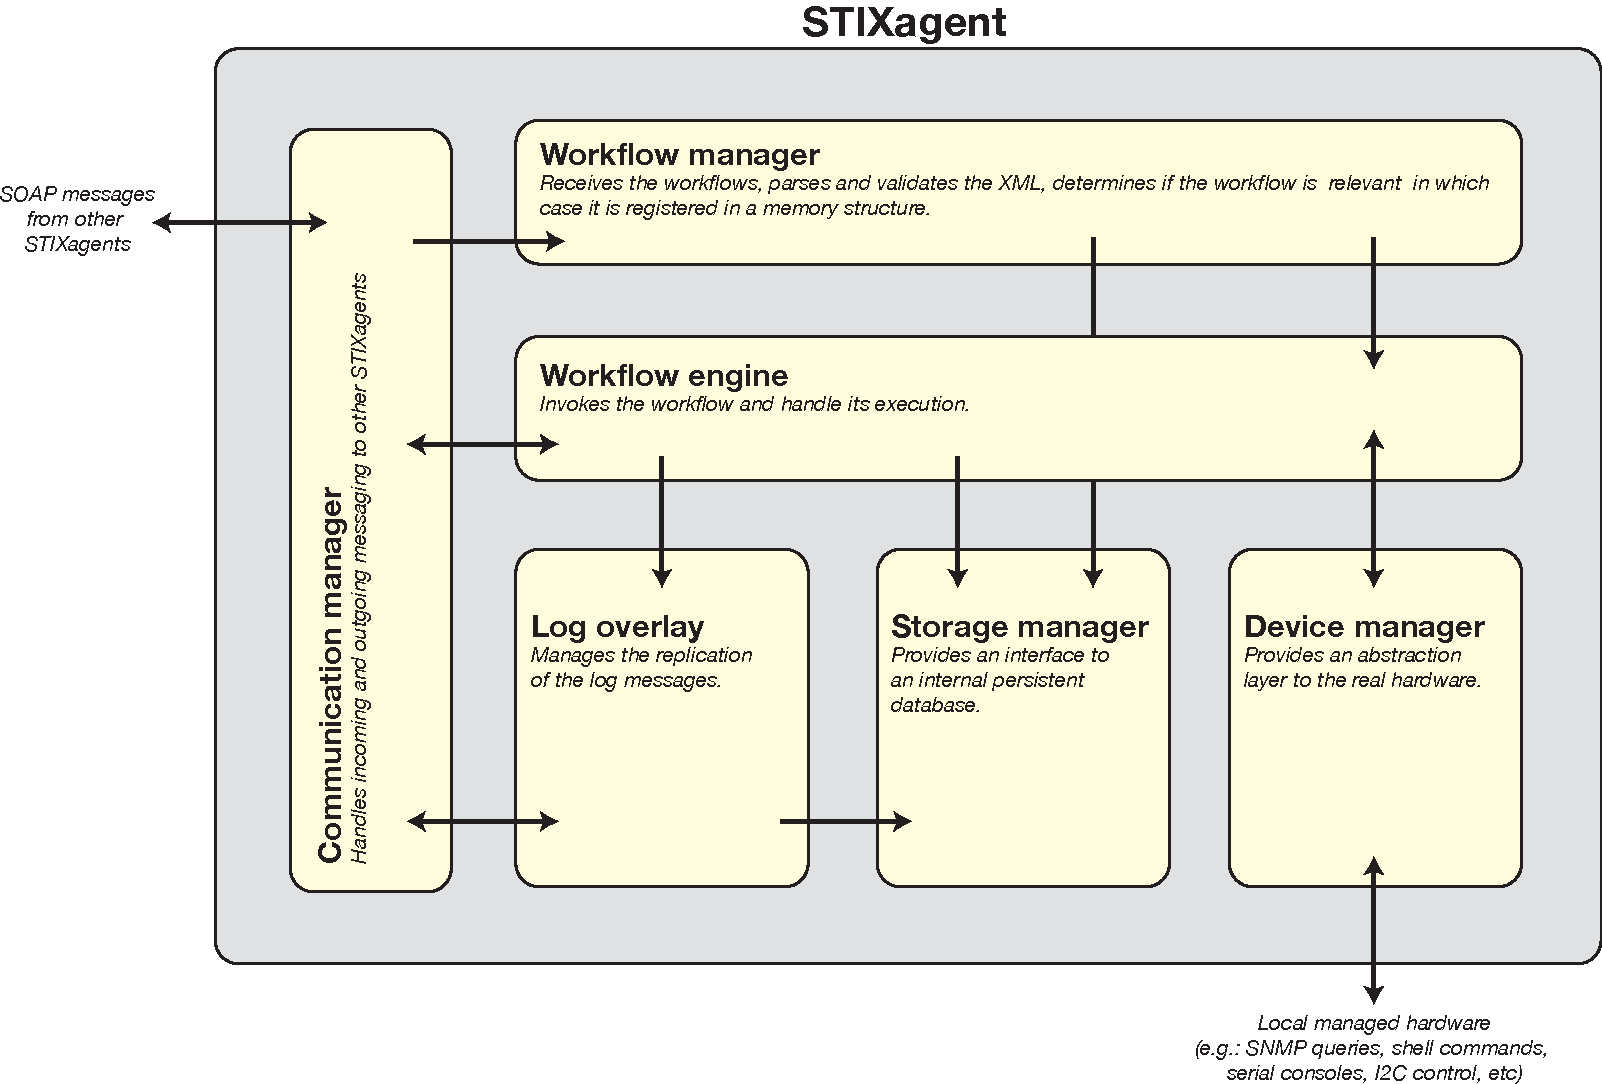
\includegraphics[width=\textwidth]{images/stixAgentComponents.pdf}
\caption{The STIXagent logical components. Arrows denote the invocation direction.}
\label{fig:stixAgentComponents}
\end{figure}

The STIXagent is composed by several elements, illustrated in Figure \ref{fig:stixAgentComponents}:
\begin{itemize}
\item a \emph{``communication manager''} that connects with other agents via SOAP messages. It listen on a network socket for incoming messages and subsequently dispatches them to the appropriate component.
\item a \emph{``workflow manager''}, which receives new workflows from the network and determines if they are `relevant' for the local connected devices. If so, it stores them to disk, transforms the XML representation in appropriate memory instructions and passes them to the workflow interpret for execution.
\item a \emph{``workflow engine''} handles the workflow execution.
\item a \emph{``log overlay''} that maintains tracks of the most recent messages originated locally or at the neighbouring sites.
\item a \emph{``storage manager''} that provides a persistent storage with an appropriate database interface.
\item a \emph{``device manager''}, which is responsible for the communication with the network device either via Operating System tools in case the STIXagent is running as a software agent on the device itself, or via a management protocol.
\end{itemize}

\label{sec:grammar}
\section{Notational Conventions and Grammar}
This section explains how to model the network management processes in the form of workflows following the NPMN syntax. An NPMN workflow is made up of a set of graphical elements which definition was originally inspired from the BPMN 1.2 standard. The important difference between BPMN and NPMN is that in the former arrows represent mere sequence flow while in the latter they depict data flow from subsequent elements.

\mnote{insert a paragraph introducing the 3 types of events, as in the BPMN specs}

\subsection{NPMN Elements}
\mnote{add further details about each of them} The components accepted in NPMN diagrams are the following. This section presents their graphical appearance and a sample of the XML code they correspond to.

\subsubsection{Pool}
It acts as a container for the events of a single workflow. In order to select the devices on which the workflow will be applied it allows to define a query expression in the left-hand vertical space.

\emph{Graphical representation:}
\begin{figure}[h!]
\centering
\includegraphics[width=0.7\textwidth]{images/pool.png}
\end{figure}

\emph{Example of XML representation:}
\begin{lstlisting}[language=XML]
<pool query="ON BTS DO" x="100" y="300" ID="stix-100" >
	...
</pool>
\end{lstlisting}

\subsubsection{Task}
A task is an individual unit of work.

\emph{Graphical representation:}
\begin{figure}[h!]
\centering
\includegraphics{images/task.png}
\end{figure}

\emph{Example of XML representation:}
\begin{lstlisting}[language=XML]
<task class="uk.ac.ed.inf.wimo.stix.doSomething" ID="stix-101" x="100" y="300">
	<flowMapping>
		<out>stix-100</out>
	</flowMapping>
	<dataMapping>
		<in>
			<parameter>
				<name>coolParameterOne</name>
				<attribute>var1</attribute>
			</parameter>
			<parameter>
				<name>coolParameterTwo</name>
				<value>1122334455</value>
			</parameter>
		</in>
		<out/>
	</dataMapping>
</task>
\end{lstlisting}
	
\subsubsection{Text annotation}
Any object can be associated a text comment to provide additional documentation.

\emph{Graphical representation:}
\begin{figure}[h!]
\centering
\includegraphics{images/text_annotation.png}
\end{figure}

\emph{Example of XML representation:}
\begin{lstlisting}[language=XML]
<...>
	<annotation>This is a comment</annotation>
</...>
\end{lstlisting}

\subsubsection{Exclusive Gateway}
It routes the sequence flow to exactly one of the outgoing branches based on conditions. When merging, it awaits one incoming branch to complete before triggering the outgoing flow.
It is the equivalent of a ``if() {...} else {...}'' instruction in a traditional programming language.

\emph{Graphical representation:}
\begin{figure}[h!]
\centering
\includegraphics{images/exclusive_gateway.png}
\end{figure}

\emph{Example of XML representation:}
\begin{lstlisting}[language=XML]
<exclusiveGateway ID="stix-100">
	<flowMapping>
		<out condition="x==1">stix-101</out>
		<out>stix-102</out> <!-- this is the else branch -->
	</flowMapping>
</exclusiveGateway>
\end{lstlisting}

\subsubsection{Inclusive Gateway}
When splitting, one or more branches are activated based on branching other conditions evaluate to conditions. When merging, it awaits all active incoming branches to complete.
It is the equivalent of a series of individual ``if() {...}'' on each of the outgoing branches.
\textit{\textbf{NOTE:} this symbol is not currently implemented and serves only as a reference for future releases.}

\emph{Graphical representation:}
\begin{figure}[h!]
\centering
\includegraphics{images/inclusive_gateway.png}
\end{figure}

\emph{Example of XML representation:}
\begin{lstlisting}[language=XML]
<inclusiveGateway ID="stix-100">
	<flowMapping>
		<out condition="x==1">stix-101</out>
		<out condition="x==2">stix-102</out>
	</flowMapping>
</inclusiveGateway>
\end{lstlisting}

\subsubsection{Parallel Gateway}
When used to split the sequence flow, all outgoing branches are activated simultaneously. When merging parallel branches it waits for all incoming branches to complete before triggering the outgoing flow.
It is the equivalent of a ``fork'' operation.
\textit{\textbf{NOTE:} this symbol is not currently implemented and serves only as a reference for future releases.}

\emph{Graphical representation:}
\begin{figure}[h!]
\centering
\includegraphics{images/parallel_gateway.png}
\end{figure}

\emph{Example of XML representation:}
\begin{lstlisting}[language=XML]
<parallelGateway ID="stix-100">
	<flowMapping>
		<out>stix-101</out>
		<out>stix-102</out>
	</flowMapping>
</parallelGateway>
\end{lstlisting}

\subsubsection{Start Messaging Event}
It enables the execution of a workflow to be triggered by an incoming message.

\emph{Graphical representation:}
\begin{figure}[h!]
\centering
\includegraphics{images/start_event_messaging.png}
\end{figure}

\emph{Example of XML representation:}
\begin{lstlisting}[language=XML]
<startMessagingEvent ID="stix-100" message="wakeUp">
	<flowMapping>
		<out>stix-102</out>
	</flowMapping>
</startMessagingEvent>
\end{lstlisting}

\subsubsection{Start Timer Event}
It enables the execution of a workflow to be scheduled at unique or periodic intervals in time. The event caption is a string that takes the form \emph{`every PERIOD from STARTDATE'}, meaning that the event will be triggered every \emph{PERIOD} seconds starting from the \emph{STARTDATE}.

\emph{Graphical representation:}
\begin{figure}[h!]
\centering
\includegraphics{images/start_event_timer.png}
\end{figure}

\emph{Example of XML representation:}
\begin{lstlisting}[language=XML]
<startTimerEvent ID="stix-100" timer="2012-05-30T09:00:00" period="100">
	<flowMapping>
		<out>stix-102</out>
	</flowMapping>
</startTimerEvent>
\end{lstlisting}

\subsubsection{Start Condition Event}
It enables the execution of a workflow to be started when the specified condition becomes true.

\emph{Graphical representation:}
\begin{figure}[h!]
\centering
\includegraphics{images/start_event_condition.png}
\end{figure}

\emph{Example of XML representation:}
\begin{lstlisting}[language=XML]
<startConditionEvent ID="stix-100" condition="config.ath1.snr<=10">
	<flowMapping>
		<out>stix-102</out>
	</flowMapping>
</startConditionEvent>
\end{lstlisting}

\subsubsection{Message Throwing Event}
It generates and send a message to another workflow. As soon as the message has been sent and acknowledged, the execution flow resumes.

\emph{Graphical representation:}
\begin{figure}[h!]
\centering
\includegraphics{images/intermediate_message_throw.png}
\end{figure}

\emph{Example of XML representation:}
\begin{lstlisting}[language=XML]
<messageThrow ID="stix-100">
	<flowMapping>
		<out>stix-102</out>
	</flowMapping>
	<dataMapping>
		<in>
			<parameter>
				<name>messageName</name>
				<value>wakeUp</value>
			</parameter>
			<parameter>
				<name>messageContent</name>
				<value>this is the content</value>
			</parameter>
			<parameter>
				<name>destination</name>
				<value>10.10.10.10</value>
			</parameter>
		</in>
		<out/>
	</dataMapping>
</messageThrow>
\end{lstlisting}

\subsubsection{Message Catching Event}
It receives a message sent from another workflow. It is always blocking, in other words the execution flow stops until the message is received.

\emph{Graphical representation:}
\begin{figure}[h!]
\centering
\includegraphics{images/intermediate_message_catch.png}
\end{figure}

\emph{Example of XML representation:}
\begin{lstlisting}[language=XML]
<messageCatch ID="stix-100">
	<flowMapping>
		<out>stix-102</out>
	</flowMapping>
	<dataMapping>
		<in>
			<parameter>
				<name>messageName</name>
				<value>wakeUp</value>
			</parameter>
		</in>
		<out>
			<parameter>
				<name>messageContent</name>
				<attribute>var1</attribute>
			</parameter>
		</out>
	</dataMapping>
</messageCatch>
\end{lstlisting}

\subsubsection{Timer Event}
When the workflow reaches this object, the execution flow stops for the specified period of time.

\emph{Graphical representation:}
\begin{figure}[h!]
\centering
\includegraphics{images/intermediate_timer.png}
\end{figure}

\emph{Example of XML representation:}
\begin{lstlisting}[language=XML]
<timer ID="stix-100" duration="3600">
	<flowMapping>
		<out>stix-102</out>
	</flowMapping>
</timer>
\end{lstlisting}

\subsubsection{Timeout event}
By attaching this element to a task, it is possible to set a timeout value after which the execution of the task is aborted and the execution continues along this branch.

\emph{Graphical representation:}
\begin{figure}[h!]
\centering
\includegraphics{images/timeout_event.pdf}
\end{figure}

\emph{Example of XML representation:}
\begin{lstlisting}[language=XML]
<task class="uk.ac.ed.inf.wimo.stix.doSomething" ID="stix-101" x="100" y="300">
	<flowMapping>
		<out>stix-100</out>
		<timeout duration="3600">stix-101</timeout>
	</flowMapping>
	<dataMapping>
		<in>
			<parameter>
				<name>coolParameterOne</name>
				<attribute>var1</attribute>
			</parameter>
			<parameter>
				<name>coolParameterTwo</name>
				<value>1122334455</value>
			</parameter>
		</in>
		<out/>
	</dataMapping>
</task>
\end{lstlisting}

\subsubsection{Error event}
When it is attached to a task object, it is used to start a separate flow in case of error.

\emph{Graphical representation:}
\begin{figure}[h!]
\centering
\includegraphics{images/error_event.pdf}
\end{figure}

\emph{Example of XML representation:}
\begin{lstlisting}[language=XML]
<task class="uk.ac.ed.inf.wimo.stix.doSomething" ID="stix-101" x="100" y="300">
	<flowMapping>
		<out>stix-100</out>
		<error>stix-101</error>
	</flowMapping>
	<dataMapping>
		<in>
			<parameter>
				<name>coolParameterOne</name>
				<attribute>var1</attribute>
			</parameter>
			<parameter>
				<name>coolParameterTwo</name>
				<value>1122334455</value>
			</parameter>
		</in>
		<out/>
	</dataMapping>
</task>
\end{lstlisting}

\subsubsection{End Plain Event}
Denotes the end of a workflow. If there are multiple branches concurrently in execution, they must all reach an end plain event before the workflow ends.

\emph{Graphical representation:}
\begin{figure}[h!]
\centering
\includegraphics{images/end_event_plain.png}
\end{figure}

\emph{Example of XML representation:}
\begin{lstlisting}[language=XML]
<endPlainEvent ID="stix-100" />
\end{lstlisting}

\subsubsection{Terminate Event}
When the execution flow reaches this elements, it immediately terminates, even if other branches are still executing.

\emph{Graphical representation:}
\begin{figure}[h!]
\centering
\includegraphics{images/end_terminate.png}
\end{figure}

\emph{Example of XML representation:}
\begin{lstlisting}[language=XML]
<terminateEvent ID="stix-100" />
\end{lstlisting}

\subsubsection{Log Event}
When the execution flow reaches this elements, a message is written to the log overlay. A message can be anything: a numeric value representing performance metric, a textual log entry, etc. Storing messages is useful in order to gather informations about the status of the network and to produce reporting via the use of the STIXview tool.  

\emph{Graphical representation:}
\begin{figure}[h!]
\centering
\includegraphics{images/log_event.png}
\end{figure}

\emph{Example of XML representation:}
\begin{lstlisting}[language=XML]
<log ID="stix-100">
	<flowMapping>
		<out>stix-102</out>
	</flowMapping>
	<dataMapping>
		<in>
			<parameter>
				<name>message</name>
				<value>this is the message to be logged</value>
			</parameter>
		</in>
		<out/>
	</dataMapping>
</log>
\end{lstlisting}

\subsubsection{Sequence Flow}
Defines the execution order of the activities. Specific rules determine which objects can be linked together.

\emph{Graphical representation:}
\begin{figure}[h!]
\centering
\includegraphics{images/sequence_flow.png}
\end{figure}

\subsubsection{Message Flow}
Symbolises information flow across pool boundaries, such as between two classes or instances. 
\textit{\textbf{NOTE:} this symbol is not currently implemented and serves only as a reference for future releases.}

\emph{Graphical representation:}
\begin{figure}[h!]
\centering
\includegraphics{images/message_flow.png}
\end{figure}

\subsection{NPMN Syntax Rules}
TBD (basically copy paragraph from the BPMN2.0 specs, removing references to the objects we removed from NPMN).

\label{subsec:querysyntax}
\subsection{NPMN Query Syntax}
Workflows are drawn within a Pool element, which also provides an area on the left corner to specify a query that identifies the devices to be considered. 

The query syntax is here defined in ABNF (Augmented Backus–-Naur Form), as defined in the RFC 5234. Keywords are not case sensitive and may be written in any lettercase, although uppercase is used here. 

% don't fix the tab here, they are the only way to align properly the code:
\begin{lstlisting}
query 				= 'ON' device-class ['WHERE' condition-set] 'DO';
device-class	= 'CPE' / 'BTS' / 'DEVICE' / ...;
condition-set	= condition [( 'AND' / 'OR' ) condition];
condition			= ['NOT'] attribute test value;
test					= < / <= / = / >= / > / <>;
\end{lstlisting}

The device-class ``CPE'' and ``BTS'' identify the devices in those two categories while the class ``DEVICE'' matches all the devices regardless of their type. The `attribute' field can be any of the internal parameters of the device, such as: model, region, firmware-version.

Some explicatory examples are presented here.

Returns all the BTS devices:
\begin{lstlisting}
ON BTS DO
\end{lstlisting}

Returns all the devices that are in the ``Lothian'' region:
\begin{lstlisting}
ON DEVICE WHERE region = 'Lothian' DO
\end{lstlisting}

Returns all the CPEs that have firmware-version between 4 and 5:
\begin{lstlisting}
ON CPE WHERE firmware-version > 4 AND firmware-version < 5 DO
\end{lstlisting}

\subsection{XML Representation of Workflows}
Workflows are created and edited in the STIX Graphical User Interface. When the administrator issues a deploy command, the workflow is serialized in a XML representation and sent out to the network. The following is an example of the structure of the XML file:

\begin{lstlisting}[language=XML]
<?xml version="1.0"?>
<workflow
	xmlns="http://www.wimo.inf.ed.ac.uk/stix"
	xmlns:xsi="http://www.w3.org/2001/XMLSchema-instance"
 	xsi:schemaLocation="http://www.wimo.inf.ed.ac.uk/stix stix.xsd">

	<metadata>
		<name>Workflow example</name>
		<author>Author Name</author>
		<uuid>550e8400-e29b-41d4-a716-446655440000</uuid>
		<rev>43</rev>
		<notes>This is a workflow example</notes>
		<enabled>1</enabled>
		<validity>
			<notBefore>2012-05-30T09:00:00</notBefore>
			<notAfter>2012-05-20T09:00:00</notAfter>
		</validity>
	</metadata>
	
	<attributeSet>
		<attribute persistent="true">
			<type>int</type>
			<name>var1</name>
			<value>123</value>
		</attribute>
		<attribute>
			<type>String</type>
			<name>var2</name>
			<value>foo bar</value>
		</attribute>
	</attributeSet>
	
	<pool query="ON BTS DO" x="100" y="300" ID="stix-100" >

		<startMessagingEvent ID="stix-101" x="123" y="345">
			<flowMapping>
				<out>stix-102</out>
			</flowMapping>
		</startEvent>

		<task class="uk.ac.ed.inf.wimo.stix.doSomething" ID="stix-102" x="100" y="300">
			<flowMapping>
				<out>stix-103</out>
			</flowMapping>
			<dataMapping>
				<in>
					<parameter>
						<name>ParameterOne</name>
						<attribute>var1</attribute>
					</parameter>
					<parameter>
						<name>ParameterTwo</name>
						<value>1122334455</value>
					</parameter>
				</in>
				<out/>
			</dataMapping>
		</task>
	
		<endEvent ID="stix-103" x="123" y="345" />
	</pool>
</workflow>
\end{lstlisting}

The \texttt{<metadata>} block, contains the following general information about the workflows: 

\vspace{0.2cm}
\noindent
\begin{tabularx}{\textwidth}{| p{3cm} | p{2.5cm} | p{2cm} | X | }
	\hline 
	\cellcolor[gray]{0.9} \textbf{Field:} 	& \cellcolor[gray]{0.9} \textbf{Type:} 	& \cellcolor[gray]{0.9} \textbf{Required:} 	& \cellcolor[gray]{0.9} \textbf{Description:} \\ \hline 	
	name					& String(255)		&	Yes	& Descriptive name \\ \hline 	
	author					& String(255)		&	No	& Author of the workflow \\ \hline 	
	uuid					& RFC4122			&	Yes	& Universally Unique Identifier (UUID)  \\ \hline 	
	rev						& int				&	Yes	& Revision number \\ \hline 	
	notes					& String(255)		&	No	& Descriptive notes for the workflow \\ \hline 	
	enabled					& boolean			&	No	& Whether the workflow is considered to be active or archived \\ \hline 	
	StartingFrom			& Date/time			&	No	& Timestamp the workflow will become active \\ \hline 	
	EndingOn				& Date/time			&	No	& Timestamp the workflow will be cease to be active \\ \hline 		
\end{tabularx}

The \texttt{<attributeSet>} block is used to define the variables used in the workflow. Each \texttt{<attribute>} defines the variable type, its name and an optional initial value. 

The remainder of the file XML is represented by the \texttt{<pool>} object and the elements defined in it. The XML is validated with an XML Schema before being sent out on the network and as soon as it is received by the agents.

\label{sec:pickandforward}
\section{`Pick and Forward' Workflow Distribution Mechanism}
As described in Section \ref{subsec:querysyntax}, the query syntax expressed in the Pool object can be used to specify which agents are meant to execute a workflow. At run-time, each node evaluates the query string contained in the Pool object in order to determine whether the particular workflow is to be considered for execution. Since queries can involve fields that can change over time, at the time a workflow is distributed a agent has no way to determine whether it needs to save it for future use and if it will ever be executed. 
\mnote{should we add an example?}

The distribution mechanisms works like this:
\begin{enumerate}
\item every STIXagent already knows about other agents that are directly connected, for example at sites to which we have a direct link to.
\item when the administrator, using the GUI, saves the workflow, it is sent to a few agents \mnote{"to a few agents"?} on the network.
\item when an agent receives the workflow, it evaluates the ``uuid'' and ``rev'' fields in its header:
\begin{itemize}
\item if the workflow has already been received, do nothing.
\item if the workflow has not been received yet, insert the ``uuid'' and ``rev'' in the local list of the last x workflow received and forward it on every link except the incoming one (split horizon technique)  
\end{itemize}
\item at this point, the agent decides whether the workflow is needed using the ``pick and forward'' technique explained below.
\end{enumerate}

The pick and forward technique uses simple heuristics to determine whether a agent should pick up and locally store a workflow passing by. A workflow is saved if any of the following statement holds true:
\begin{itemize}
\item the \texttt{device-class} in the query matches that of one of the devices connected and there is \texttt{WHERE} statement. 
\item the \texttt{device-class} matches that of one of the devices connected and the WHERE statement operates on fields that are static or monotonic (so that the condition cannot become false).
\end{itemize}

In case one of the link is down, the agent should store the workflow until the link comes back up. Newly connected agents send a unicast query to the server in order to get the complete set of workflows. 

\label{sec:localstorage}
\section{Local storage}
Each device saves in the local memory the configuration parameters and the locally defined persistent variables. This storage is persistent and does not get lost in the event of a reboot. The minimal set of parameters and statistics to be implemented are listed in the following table:

\vspace{0.2cm}
\noindent
\begin{tabularx}{\textwidth}{| p{2cm} | p{2cm} | X | }
	\hline 
	\cellcolor[gray]{0.9} \textbf{Field:} 	& \cellcolor[gray]{0.9} \textbf{Type:} 	& \cellcolor[gray]{0.9} \textbf{Description:}\\ \hline 	
	hostname				& rw				& Hostname of the device \\ \hline 	
	date					& rw				& Current date \\ \hline 	
	...						& ...				& ... \\ \hline 	
\end{tabularx}

\label{sec:events}
\section{Events}
An event in NPMN represents that ``something has happened'' in the network, so that an appropriate action can be taken. Using the ``start condition event'', workflows can be triggered by various actions. The following list represent a minimal mandatory set to be implemented in the agent:

\vspace{0.2cm}
\noindent
\begin{tabularx}{\textwidth}{| p{4cm} | X | }
	\hline 
	\cellcolor[gray]{0.9} \textbf{Name:} 	& \cellcolor[gray]{0.9} \textbf{Description:} \\ \hline 	
	new\_cpe\_connected 	& A new CPE device is connected. \\ \hline 	
	new\_bts\_connected		& A new BTS device is connected. \\ \hline 	
	timer					& A timer is triggered. \\ \hline 	
	message\_received		& A message has been received. \\ \hline 	
	startup					& The device has completed the boot procedure. \\ \hline 	
	shutdown				& The device is about to start the shutdown procedure. \\ \hline 	
	...						& ... \\ \hline 	
\end{tabularx}

\label{sec:loglayer}
\section{Log layer}
By using the ``log event'' object, workflows can save messages containing information on their execution, log messages, performance statistics, etc. These messages are automatically stored in a network overlay which is aware of the network topology and is optimised for low-overhead and redundancy.

A message is defined as a tuple on the following five attributes:
\begin{lstlisting}
{AgentID, WorkflowID, Name, Value, Timestamp}
\end{lstlisting}
AgentID and WorkflowID are the unique identifiers of the node that initiated the log operation, Name is an arbitrary string that identifies the type of message, Value is the content and Timestamp represents the date and time the message was generated.

When a workflow invokes the ``log event'', the agent saves the message locally and sends the message to the directly connected neighbours. The underlying principle is the following:
\begin{itemize}
	\item an agent stores all the messages generated locally up to a configurable \texttt{prune\_period}.
	\item the \emph{j}-hop neighbours store the last \texttt{jnum} messages.
	\item the \emph{k}-hop neighbours store the last \texttt{knum} messages.
\end{itemize}
A good value for \emph{j} and \emph{k} may be 1 and 3 with decreasing values of \emph{jnum} and \emph{knum} (such as 100 and 30), so that even in the case an agent becomes unreachable, the administrator is still able to access and investigate its logs by consulting its neighbours. Storing data also on more distant neighbours (3-hop in this example) helps in case a larger section of the network goes down. As an example, consider the topology of Figure \ref{fig:logoverlay}, relative to the messages generated by SiteA, with the following configuration values: j=1, k=2, jnum=5, knum=3.

The multiple-replication scheme described exploits the particularities of WISPs networks avoiding the complexities and traffic overhead of full-blown data replication algorithms, as follows. First, by storing data on neighbouring sites that have a mutual physical connection, we limit the network utilisation to the minimum. Also, since the failure of a single wireless link may result in a larger region of the network being unavailable, replicating data a few hops away from its source increases the probability of being able to access it at all times. 

\begin{figure}[h!]
\centering
\includegraphics[width=\textwidth]{images/logOverlayExample.pdf}
\caption{Example of log overlay}
\label{fig:logoverlay}
\end{figure} 

\label{sec:tasklibrary}
\section{Tasks Library and Hardware Abstraction}
A task is an elementary unit of work. The STIX user can define new ones, import them from third parties or grab existing ones from a library. Stencils are global and, once installed, they are available throughout the network. In a workflow, tasks have input and output parameters.

Examples of tasks are the following:

\vspace{0.2cm}
\noindent
\begin{tabularx}{\textwidth}{| p{4cm} | X | }
	\hline 
	\cellcolor[gray]{0.9} \textbf{Name:} 	& \cellcolor[gray]{0.9} \textbf{Description:} \\ \hline 	
	send\_email				& Send an email. \\ \hline 	
	reboot					& Reboot the device. \\ \hline
	get\_bts\_list			& Gets the list of BTSs available. \\ \hline
	get\_cpe\_list			& Gets the list of CPEs connected. \\ \hline
	...						& ... \\ \hline 	
\end{tabularx}

Tasks don't access directly to the hardware, instead they call a set of internal methods that abstract the underlying hardware and provide a common interface regardless of the device type and vendor. 
\mnote{Identify the list of methods?}

\subsection{Stencil exchange format}
TDB. (Provide details of the binary format, including code signature, but it is pointless to do this now)

\label{sec:gui}
\section{GUI - Graphical User Interface}
The system interface, called STIXgui, is a web-based application that runs on the server and is composed of four main screens. This section presents a prototype view and a basic explanation of the interaction mechanisms.

The first screen, shown in Figure \ref{fig:gui1}, presents a \emph{topology view} in which the STIXagents are linked together to give a glance of the network layout. A link is shown between two sites when there is a link between them. When a node is clicked, the view is expanded and the locally installed devices are shown. Clicking on a device opens a menu that allows to manually change its configuration and to see the list of workflows that affect that device.

The second tab, in Figure \ref{fig:gui2}, is a simple inventory that lists the workflows defined in the system. A row for each of them states their name, a brief description, their revision number and other optional details. From this screen it is possible to open the \emph{process edit window} (Figure \ref{fig:gui3}), to edit, delete and create new workflows. The view is divided into three panels: on the left the \emph{task library} with the list of NPMN events and tasks imported in the system, on the top-right the \emph{flow mapping} pane to compose the active workflow and wire events and tasks in sequence. As soon as a task is selected in the flow mapping window, the bottom pane shows its current \emph{data mapping}. Through this visualisation the administrator can map workflow variables to input and output parameters.

Finally, Figure \ref{fig:gui4} shows the \emph{STIXview} component: a flexible realtime reporting system that can be used to document network processes and to investigate the current operational status. On the left pane, `perspectives' can be selected, created and deleted. When a perspective is selected, the right side of the window becomes an initially blank page which can be edited in a wiki-like fashion using a common markup syntax. A perspective is just like a traditional document that can contain static text and images, or it can include queries to the `log overlay' presented as text, graphs or as a list of records. The following are examples of what the query syntax can specify:
\begin{itemize}
	\item select the last 10 log entries for any PTP device in a network region, and show them in a table.
	\item plot a pie graph of the percentage of completed and failed firmware upgrade over the last day.
	\item print a number representing the average SNR value of a link over the last hour.
\end{itemize}
Perspectives can be edited by any user, previous versions are kept accessible as an option.

The syntax of the wiki pages may contain the following markup codes:
\vspace{0.2cm}
\noindent
\begin{tabularx}{\textwidth}{| p{4cm} | X | }
	\hline 
	\cellcolor[gray]{0.9} \textbf{Markup:} 	& \cellcolor[gray]{0.9} \textbf{Meaning:} \\ \hline 	
	\texttt{''text''}		& Italic text \\ \hline
	\texttt{''''text'''}	& Bold text \\ \hline
	\texttt{= Text =}		& Section header \\ \hline
	\texttt{== Text ==}		& Subsection header \\ \hline
	\texttt{=== Text ===}	& Sub-subsection header \\ \hline
	\texttt{[[Text]]}		& Link to another perspective \\ \hline
	\texttt{* Text \newline ** Text \newline * Text \newline * Text}	& Unordered lists. More stars indicate a deeper level. \\ \hline
	\texttt{# Text \newline ## Text \newline # Text \newline # Text}	& Numbered lists. More hash symbols indicate sub-numbering. \\ \hline
	\texttt{\{\{\{ QUERY \}\}\}}	& Insert query and present the result as field, table or plot. \\ \hline
\end{tabularx}

By using the notation \texttt{\{\{\{ON ... SELECT ...\}\}\}}, dynamic data can be integrated in the visualisation. The query syntax allowed follows this ABNF notation: 

% don't fix the tab here, they are the only way to align properly the code:
\begin{lstlisting}
query 					= 'ON' (list-of-agents / '*')
						   	'SELECT' (field / list-of-fields / '*')
						   	['WHERE' condition-set]
						   	['ORDER BY' field ['ASC' / 'DESC']]
						   	['LIMIT' 1*DIGIT]
						   	'PRESENT AS' ('FIELD' / 'TABLE' / 'PIEGRAPH' / 'BARGRAPH' / 'LINEGRAPH');
condition-set		= condition [( 'AND' / 'OR' ) condition];
condition				= ['NOT'] field test value;
test						= < / <= / = / >= / > / <> / 'LIKE';
field						= agentid / workflowid / name / value / timestamp
list-of-fields	= 1*(field ',')
\end{lstlisting}

For example, this query renders a line graph of the SNR value recorded on a link:
\begin{lstlisting} 
ON siteOne
SELECT value
WHERE name = 'SNR' AND workflowid = 'test123'
ORDER BY timestamp DESC
PRESENT AS LINEGRAPH;
\end{lstlisting}

At render-time, the server interprets the markup syntax of the page and it analyses the queries specified. For each of them, the software determines whether the data has to be collected from a single agent (i.e. if a \texttt{ON agent} is specified) or from many and it sends out queries to the communication manager of those remote agents. Results are aggregated and rendered as a field, a table or a plot. In case an agent is not responding to the query, the software on the server tries to collect the same data from the neighbours of the unreachable agent, following the `Log overlay' paradigm described in section \ref{sec:loglayer}.

\begin{figure}[h!]
\centering
\includegraphics[height=13.5cm, angle=90]{images/stixGUI_1.pdf}
\caption{tbd}{\emph{Topology} tab of the GUI}
\label{fig:gui1}
\end{figure}


\begin{figure}[h!]
\centering
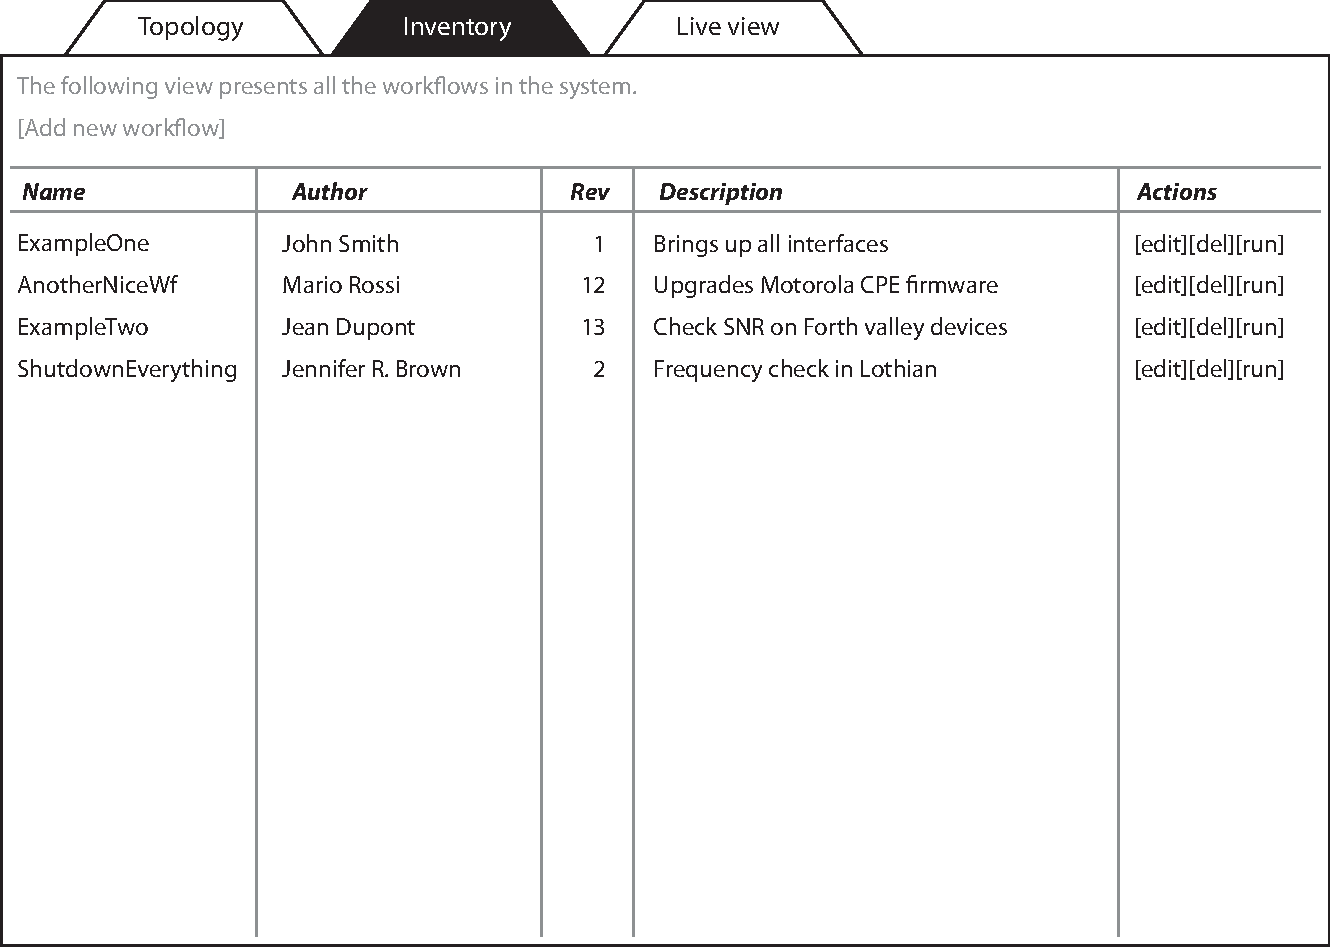
\includegraphics[height=13.5cm, angle=90]{images/stixGUI_2.pdf}
\caption{tbd}{\emph{Inventory} tab of the GUI}
\label{fig:gui2}
\end{figure}


\begin{figure}[h!]
\centering
\includegraphics[height=13.5cm, angle=90]{images/stixGUI_3.pdf}
\caption{Process edit window}
\label{fig:gui3}
\end{figure}


\begin{figure}[h!]
\centering
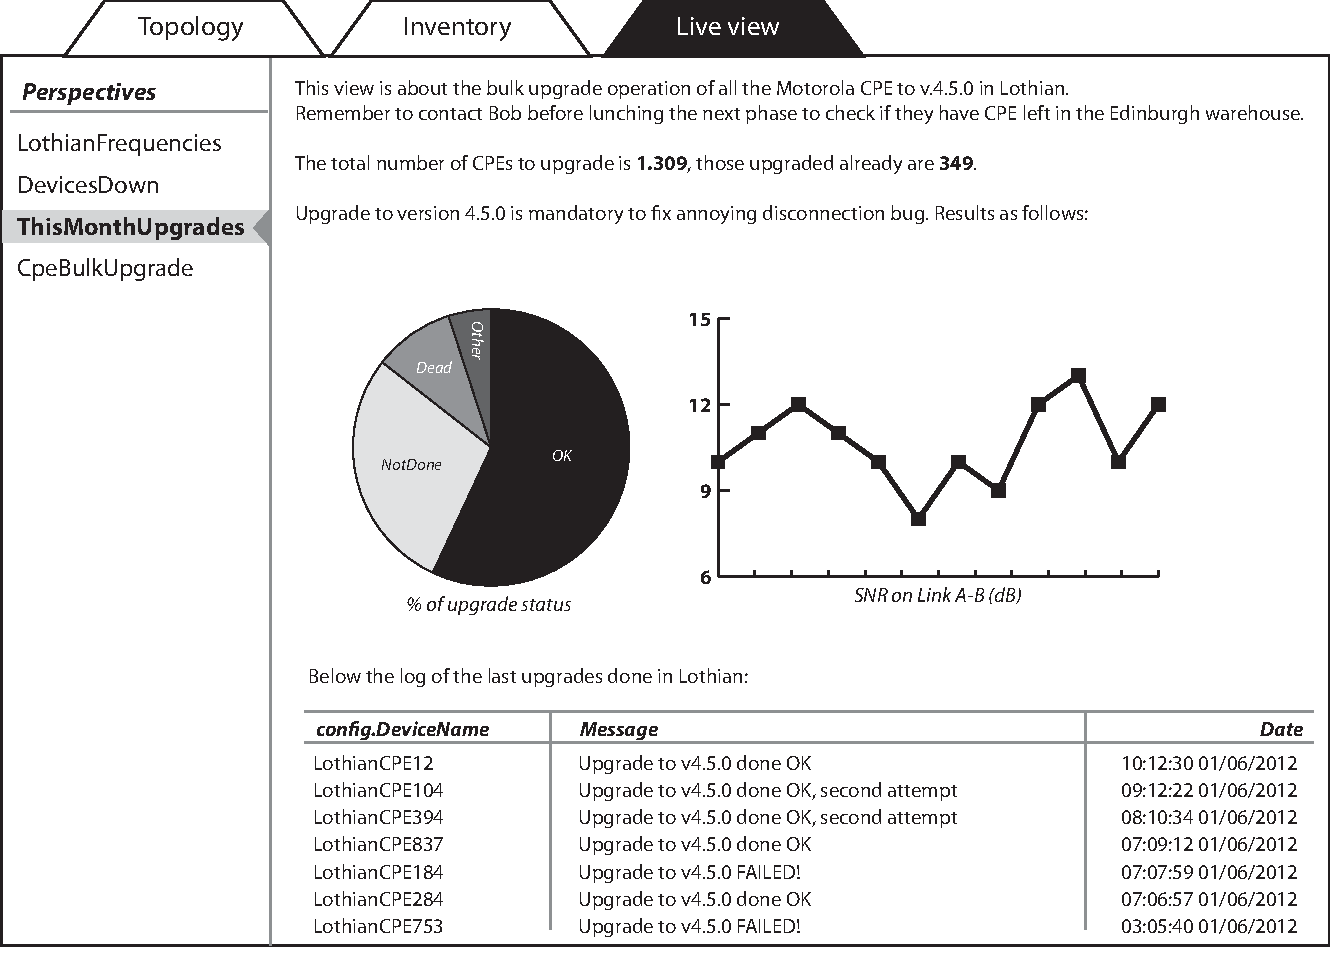
\includegraphics[height=13.5cm, angle=90]{images/stixGUI_4.pdf}
\caption{STIXview interface}
\label{fig:gui4}
\end{figure}

\clearpage
\label{sec:stixcontrol} 
\section{STIXcontrol interface}
In order to give the administrator the possibility of remotely controlling the hardware, the STIXcontrol board can be used. It is an embedded adapter that sits between a device and its power supply and allows to:
\begin{itemize}
	\item read realtime current consumption (in Amps)
	\item read realtime voltage (in Volts)
	\item perform power off, power on and power cycle 
\end{itemize}
STIXcontrol is equipped with a Current sensor, an 8-channel 12-bit ADC, a relay and a I2C interface. Up to 8 STIXcontrol can be daisy-chained on an I2C bus to a single STIXagent, as in the example in Figure \ref{fig:hardware}.

\mnote{insert schematics when Rob will provide them}
Current and voltage sensors can be read and the relay can be operated using a specific task object.

\begin{figure}[h!]
\centering
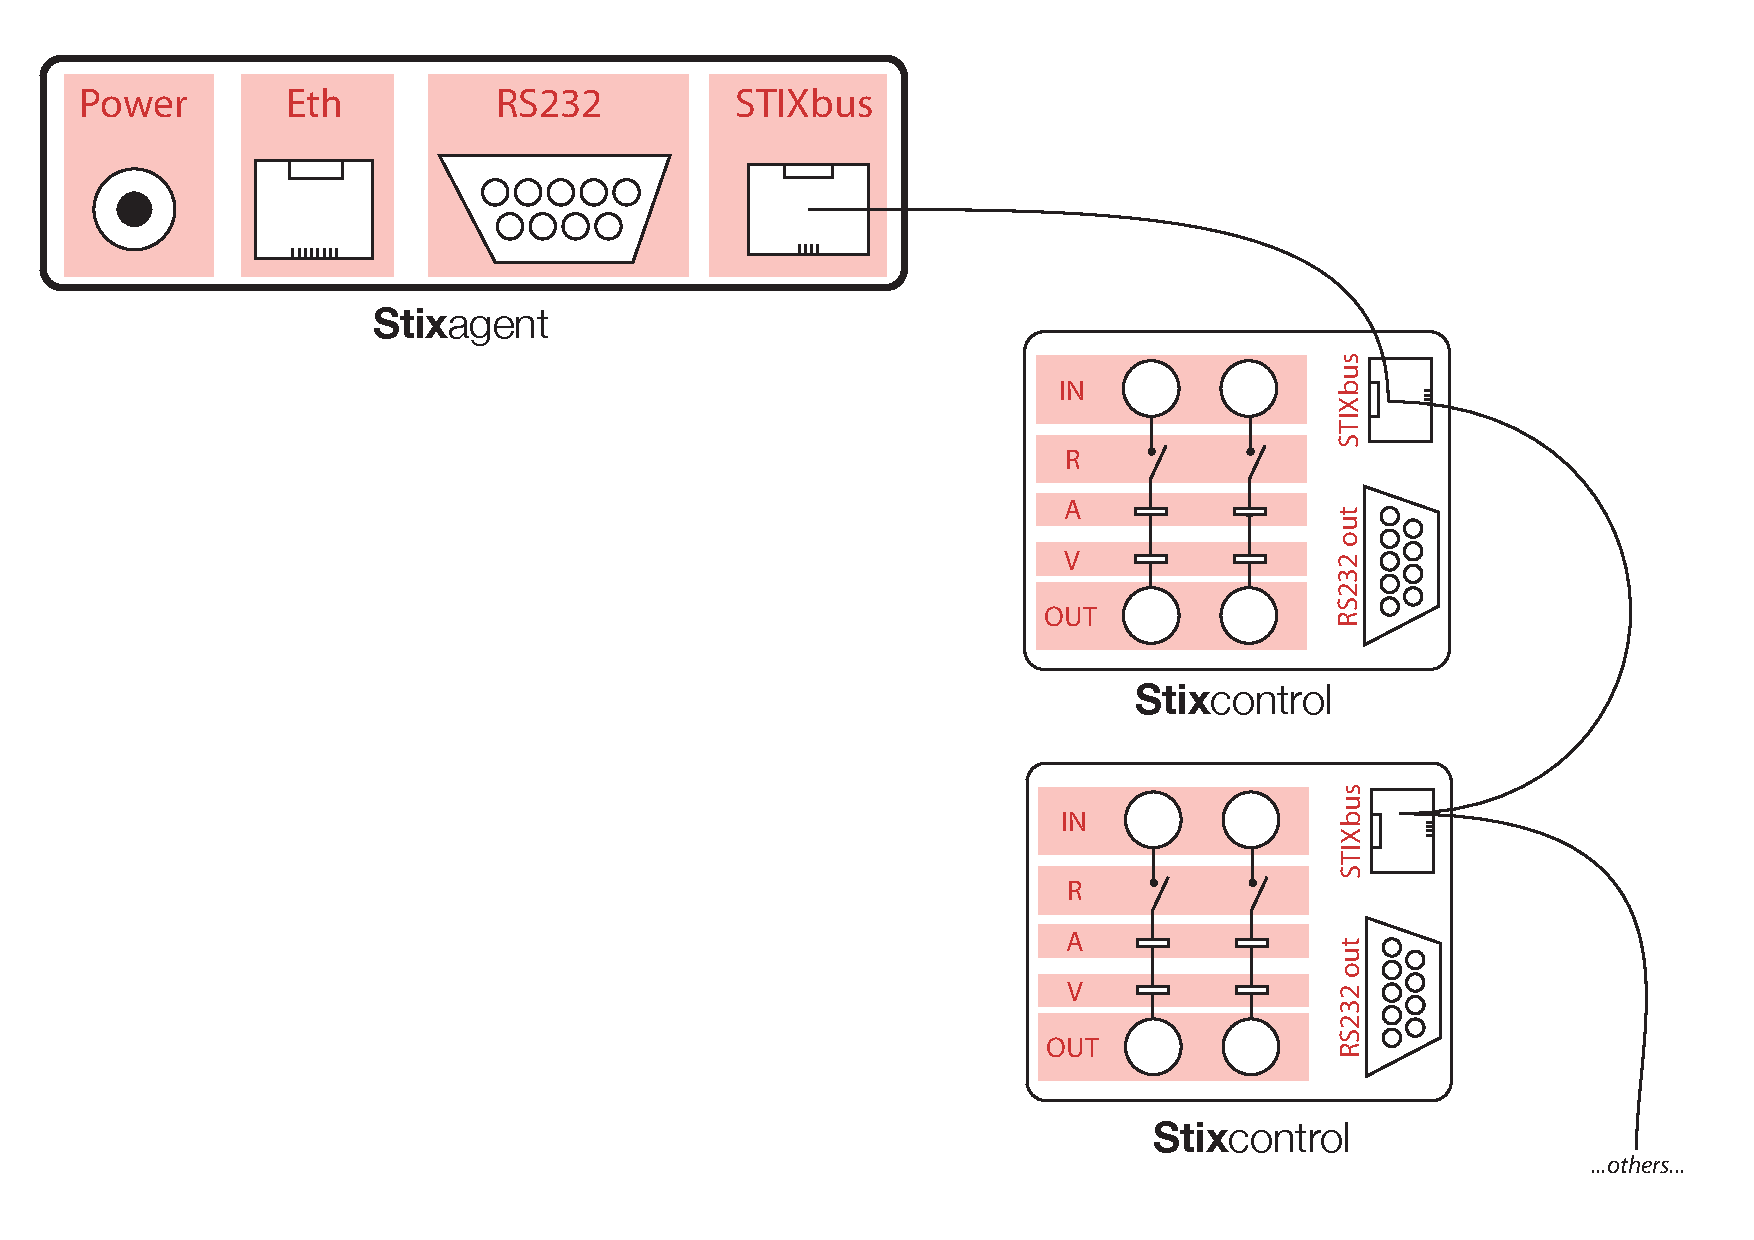
\includegraphics[height=13.5cm, angle=90]{images/stixDrawings_1.pdf}
\caption{Connection layout of STIXagent and STIXcontrol}
\label{fig:hardware}
\end{figure}

\clearpage
\label{sec:agentcomponents}
\section{STIXagent components}
This section provide a guideline about the implementation of the STIXagent software. As previously shown in Figure \ref{fig:stixAgentComponents}, the agent software is composed by six independent modules which are here described.

\subsection{Communication manager}
This component is responsible for any data exchange that happens over the network between STIXagents. It listens on a TCP socket expecting incoming SOAP messages, which may contain new workflows, new log entries to be stored, or requests for previous log entries. Once the message has been received, it is dispatched to the relevant internal component, for example messages containing workflows are forwarded to the Workflow Manager while log messages are sent to the Log Overlay.

The component provides the following interfaces:
\begin{itemize}
	 \item \texttt{sendMessage(DestinationAgent, Message)}: invoked with the identifier of another STIXagent and the message content.
\end{itemize}

\subsection{Workflow manager}
It receives new workflows and applies the `pick and forward' technique, described in Section \ref{sec:pickandforward}, in order to determine if they are relevant for the locally connected components. If so, the workflows are stored and passed to the interpret.

The component provides the following interfaces:
\begin{itemize}
	 \item \texttt{receiveWorkflow(WorkflowXML)}: it is invoked by the Communication Manager when a new workflow has been received from another agent.
\end{itemize}

The steps performed by the workflow managers are the following:
\begin{lstlisting}
// Perform some simple validation:
1. check the XML against the XML Schema
2. if the number of start_event is != 1, throw error ad abort.
3. if the number of end_event is == 0, throw error ad abort.
4. check that the workflows have no null outgoing links.
5. (... other checks to be done TBD ...)
6. forward to the Workflow interpret

7. Forwarding to the neighbours:

// Check if the workflow is relevant:
8. analyses the query syntax to check whether it's relevant for the current agent:
	8.1. if not: discard the workflow and terminate
\end{lstlisting}


\subsection{Workflow engine}
It is the engine that is responsible for parsing, scheduling and interpreting the NPMN processes.

A process language (such as a workflow-based language) is nothing more than a set of `nodes' implementations, `tasks' in our case. A Java taskObject class can be provided as a set of abstract interfaces which implementation becomes mandatory. When the execution flow reaches a tasks, we say that that particular task is activated, and its execute() method is called. In this way, the semantics of each task are defined by the implementation of the execute() method in the respective task class.

The way the interpret parses the workflows and handle their execution is crucial and must be carefully developed, as there could be a significant number of workflows concurrently running on a single agent. At a high level of abstraction, the general task can be handled as follows:

\begin{lstlisting}
// Register the workflow:
1. find the start_event and identifies what condition starts the workflow (e.g.: trigger, timer, manual).
2. add the workflow to a linked list of workflows (the `workflows register').
3. generate a multiple-linked list in memory of the workflow objects, where links represents edges on the workflow.
...
\end{lstlisting}

Another thread of the program is continuously cycling in the workflow register� and evaluating if the starting condition is true. If it is, it will start running that workflow by following the edges and calling the execute() method of each task.

The component provides the following interfaces:
\begin{itemize}
	\item \texttt{receiveMessage(SourceAgent, Content)}: it is invoked by the Communication Manager when a message, generated by a `Message Throw' event on another agent, is received.
	\item \texttt{registerNewWorkflow(WorkflowXML)}: it is invoked by the Workflow Manager when a new workflow is to be registered in memory.
	\item \texttt{conditionTriggered(ConditionID)}: called by the Device Manager when a condition, previously registered with the \texttt{registerCondition()} method, becomes true. The identifier \texttt{ConditionID} is attached to the callback to allow identification of the workflow associated with the callback.
\end{itemize}

\subsection{Log overlay}
It implements the log overlay mechanism described in Section \ref{sec:loglayer}, interfacing with the Communication manager, the Storage manager and the Workflow interpret.

The component provides the following interfaces:
\begin{itemize}
	 \item \texttt{queryLog(QuerySyntax)}: executes QuerySyntax on the local query log and returns the resulting recordset.
	 \item \texttt{writeLog(Agent, Workflowid, Name, Value, Timestamp)}: writes a new message in the log.
\end{itemize}

\subsection{Storage manager}
It provides an interface to the internal persistent storage, which is structured as a database system.

The component provides the following interfaces:
\begin{itemize}
	\item \texttt{query(SqlQuery)}: executes SqlQuery on the local storage and returns the resulting recordset.
	\item \texttt{writeWorkflowXml(WorkflowXML)}: saves the workflow XML representation.
	\item \texttt{readWorkflowXml()}: returns an array of the XML code of all the workflows in the system.
	\item \texttt{readWorkflowVariable(WorkflowID, Name)}: returns the workflow variable identified by WorkflowID and Name.
	\item \texttt{writeWorkflowVariable(WorkflowID, Name, Value)}: write the workflow variable value on the local storage.
	\item \texttt{readDeviceVariable(Name)}: returns the device variable identified by Name.
	\item \texttt{writeDeviceVariable(Name, Value)}: write the device variable value on the local storage.
\end{itemize}

\subsection{Device manager}
It is responsible for communicating with the actual hardware over a suitable protocol, for example SNMP, Telnet, a serial console interface, etc.

The component provides a number of interfaces that implement the hardware abstraction level described in Section \ref{sec:tasklibrary}, plus the following ones:
\begin{itemize}
	\item \texttt{registerCondition(Condition)}: it registers a \texttt{Condition} and returns an ID for that condition. When this becomes true the method \texttt{conditionTriggered} of the workflow engine is called with the specific ID as argument.
\end{itemize}

\clearpage 
\label{sec:usecases}
\section*{Appendix A: Definition of scenarios and use cases}

\mnote{Completely discard this section, for now.}The following section presents three use cases and provides the details of the key challenges they pose. By analysing the following set of scenarios we try to stress that many problems have to be tackled differently in the wireless domain, compared to traditional wired networks. The high complexity and the large quantity of parameters in current wireless implementations often demands for a deeper knowledge of the network topology and of the peculiarity of each class of devices in order to achieve good performance. Also, mobile networks are dynamic structures in which new sites are continuously new sites deployed, capacity extensions are made and parameters are adapted to local conditions.

The ideal ``actor'' behind these use cases is the network administrator of a Wireless Internet Service Provider (WISP), of a large organisation with wireless deployments or of a community-driven wireless deployment. While the scope of such networks is centred on IP access, we are also interested in future 4G/LTE platforms, which will soon represent massive deployments in many countries.

\subsection*{Scenario 1: Remote configuration management}
\subsubsection*{Network environment}
In modern carrier-grade wireless devices, an increasingly large part of functionalities is implemented in firmware. Vendors rely on firmware upgrades mechanisms to improve the performances, fix bugs or add new features to devices already on the market without occurring in the costs of an hardware redesign.

The growing size of the configuration parameter space is an unavoidable characteristic of increasingly intelligent devices. As new functions are added and novel services get supported, more and more variables are introduced to control the device. This increase the demand for seamless configuration management mechanisms. 

\subsubsection*{Key Challenges}
The main challenge in changing the software running on remote wireless devices is the lack of out-of-band channels to reach and control the device. Operations such as firmware upgrades or reconfiguration perform critical operations on the onboard memory and thus have an inherent risk of loosing control of the device. Complex network topologies suggest that the unavailability or misbehaviour of a single device can disrupt wider regions of the network or interfere with seemingly unrelated services.

Network scale poses a strong operational challenge, as the number of devices to be upgraded or reconfigured can be very large. As an example, the upgrade of all the CPEs installed by an Internet Provider may require the download on the device of a binary image of a few megabytes prior to the operation. If the upgrade is simultaneously started for the whole network, the firmware repository may undergo a very heavy load and become unresponsive.

\subsubsection*{Detailed use case description}
It is often necessary to upgrade the firmware of network devices in order to fix critical bugs or implement new features. The upgrade procedure is different depending on the role of the device. In case of BTSs, the network administrator has to first re-route the network traffic to other nodes that will not be upgraded immediately. It is then possible to start the upgrade procedure, for example by sending a binary image of the embedded memory or by modifying the filesystem, which are operations that present an inherent risk of loosing control. The last step is to reboot, reload or apply the modifications and to check whether the upgrades has completed successfully. If that is the case, the procedure is repeated for the subsequent BTSs.
For CPEs upgrades, the task can become even more complex as these devices are housed at the subscriber site so they can be powered off at any time and can remain off for an arbitrary period (e.g.: customer on holiday). The task of programming all the devices becomes thus indefinitely long, and the system has to periodically check whether CPEs with the previous version of the firmware join the network in order to upgrade them.

The series of steps described is certainly not scalable in relation to the number of devices, especially if it involves manual actions to be performed (e.g.: traffic re-routing, backups, etc). However, it offers some degree of parallelization as upgrades can be performed on several devices in different areas of the network at the same time. 

\subsubsection*{Further use cases}
\noindent\emph{Scenario 1.1: Remote hardware control}

When sensitive operations, such as firmware upgrades, have to be performed, it may prove useful to be able to remotely control the devices for example by performing so-called ``power operations'' (i.e., reboot or shutdown) or by connecting to a debugging interface (i.e., serial or JTAG). Enabling such functionalities in a management framework is like providing ``remote eyes and hands'' to the network administrator, giving him the ability of restore a remote device like it was handled locally. This feature is of even greater importance for ISPs operating in rural regions, where reaching the deployed devices can be problematic. 

\noindent\emph{Scenario 1.2: Bulk configuration change}

Sometimes the administrator needs to change one or more configuration parameters in bulk on all or a specific subset of devices. For example, he may decide to lower the bitrate of all the CPEs that present a signal strength lower than a threshold, or to reboot all the BTSs running a specific software version. It should be possible to base the selection on any parameter, such as the type of device (i.e.: BTS or CPE), the type of contract the subscriber is entitled, the network address, the geographic area, etc. Also, since CPEs can be powered off at any time, he needs to be sure that the configuration is applied once the device comes back online. He would like the network management system to do this automatically.

\noindent\emph{Scenario 1.3. Warehousing and logistics in the deployment of new devices}

Each time the network coverage in a specific area is expanded or improved, there is a significant amount of equipment involved: new BTSs are installed, CPEs are sent out to the new subscribers. The network administrator has to allocate network resources to each of these devices, such as frequencies and IP addresses, and configure them either prior to their installation or at their first connection attempt. He would like the management system to track these myriad of components and configure them when needed.

\subsubsection*{State of the art and limitation of current approaches}
tbd

\subsubsection*{Our approach and expected benefits}
tbd

\subsection*{Scenario 2: Regional frequency management}
\subsubsection*{Network environment}
The scarcity of the radio spectrum makes it impossible to allocate a unique radio channel to each wireless ``cell'' (e.g. BTS) of the network, thus a frequency reuse policy is needed. When two or more radio devices within reach are transmitting on the same frequency, interference is generated and can cause performance degradation. The need for a valid frequency planning is always true, regardless of the regulatory state of the spectrum: even if the operator is using a licensed band, he will have to carefully divide it and to assign it to devices. The same is for unlicensed spectrum, for which devices belonging to other operators have to be considered as well.

\subsubsection*{Key Challenges}
Frequency planning has to take into account a wide number of factors including devices location, geographic characteristics, number of customers in the area and so on. Traffic demands also vary according to the time of the day, the day of the week and the time for which the region has been served.

Any planning mechanism must support the growth of the network, such as identifying when a new device is added and adjust the network automatically to optimise. Considering equipment of different vendors the situation gets even worse, as they may support different performance counters and measurements. Network operators have to develop adaptation layers to translate the performance measurements from different vendors such that a common optimisation platform can be used. 

\subsubsection*{Detailed use case description}
We consider an ISP operating in the unlicensed spectrum that has to subdivide the allowed band in a number of channel and to allocate them to the network cells. The operator has to design and implement frequency reuse techniques and to assign the same channel to multiple BTSes that do not mutually interfere. As predicting outdoor wireless propagation is hard and results can change over time, it is important to periodically check that there are no geographic locations covered by more than one mast operating on the same frequency, as these would represent sources of interference. A possible solution to carry out this task is to gather the list of BTSs (and their frequencies) that can be seen from each CPE and verify that they are all operating on distinct channels.

\subsubsection*{Further use cases}
This scenario suggests additional situations worth of attention in a system design perspective.

\noindent\emph{Scenario 2.1: Automatic channel monitoring/selection}

When a network is operating in the unlicensed spectrum, interference may be more likely to happen at any time, for example if other operators with equipment on the same towers start transmitting on the same frequencies. In this case, the ``best practice'' is to have PTP devices to periodically verify the RF Noise on the frequency range supported, and to change channel if needed. It is important to note that such a ``channel hop'' should be negotiated with the remote end and that it can have consequences on the frequency allocation policy of a large part of the network.

\noindent\emph{Scenario 2.2: Forced CPE handover}

During the operation of a WISP network it may happen that some BTSes get crowded, for example as a result of marketing/sales campaigns targeted to a specific geographic region. Over time, such cells tend to receive a significant share of the network traffic and to get closer to saturation. It is a good practice to have the management system to automatically handle these situations by identifying those CPEs that can be handed to different BTSs and to force them to change their wireless association.

\noindent\emph{Scenario 2.3: Channel width adaptation}
In some circumstances it may be appropriate to adjust the channel width of existing links: this is the case of long-distance PTP links in adverse condition such as operating over water, in hostile weather, or with scarce energy left. It has been shown that reducing or increasing the channel width can be used as an effective technique to increase the Signal-to-Noise quality and save power. A tool for online frequency management could exploit this notion and adapt the configuration of PTP links accordingly. 

\subsubsection*{State of the art and limitation of current approaches}
tbd

\subsubsection*{Our approach and expected benefits}
tbd

\subsection*{Scenario 3: Alarm visualisation and escalation}

\subsubsection*{Network environment}
Wireless networks, especially large scale deployments, transform alarm management in a nightmare: a much larger parameter space compared to wired devices, different interpretation given by competing vendors on the same metrics, dynamic fluctuation of radio conditions due to external parameters are some of the unique challenges of Operation\&Management (O&M) in the BWA field.

\subsubsection*{Key Challenges}
This scenario focuses on three important concepts in network management: alarm detection, alarm escalation and alarm correlation. While there are many known techniques to handle the former, even in a feature-rich domain such as wireless networks, alarm escalation and correlation represent a challenge that requires the management framework to have a holistic knowledge of the whole network. Commercial WISPs see alarm management as a tool that can move real money, both by allowing the rollout of stricter Service Level Agreements (SLAs) and by generating savings due to lower downtime costs.

Operational challenges of this scenario include the complications of multi-vendor deployments, as different manufacturers can give different meaning to alarms and performance metrics. The scale of the deployment is itself a challenge tightly bound to the limits of centralised solutions: large deployment rule out polling mechanisms in which data is periodically ``pulled'' from the devices, and it is implausible to have a single point of collection for all the alarms generated by the devices.

Network administration presents a significant cognitive overhead: there is always something happening in a large system and constant changes due to device malfunctioning, radio interference, blackouts and a large set of other causes. As these events are by nature unpredictable, the administrators must be prepared to identify negative events, to diagnose the underlying problems and to act as fast as possible. In large organisations, there is also an additional burden of coordination with co-workers. While an administrator is actively working on an issue, the system continues to operate and may require additional support. It is important provide a tool for effective communication, documenting and reporting within the administration team, so that each member is aware of `who is doing what' to support operations.

\subsubsection*{Detailed use case description}
It is common for country-wide or even regional WISPs to scale up to ``all-wireless'' networks of hundreds or thousands of BTSes and PTP links, and order of magnitude more of CPE devices. In this context, being able to generate a realtime overall map of the network is very useful to understand the status of the deployment at a glance and point out anomalies. This functionality, which is often called ``weather map'', gives the network administrator information about possible problems at a glance, thus providing a valid help in troubleshooting. Despite they have been long used in several fields of industry and commerce and have been studied in the context of information graphics, they are still relatively an unexplored resource in the domain of wireless networks. In general, the ability of effectively presenting a very large parameter space is itself an invaluable tool in the hands of network administrators.

\subsubsection*{Further use cases}
\noindent\emph{Scenario 3.1: Power monitoring} 

Wireless ISPs operating in rural regions are often faced with the challenges of deploying devices in strategic locations which are far from energy sources. The energy subsystem of self-powered masts can represent the most significant part of the financial expenditure, so it is important to determine the right scale to avoid over-provisioning it. An effective monitoring system should take self-powered masts into consideration and control the health status of the batteries (e.g., compared to historical data), the remaining power and provide the network administrator a feedback when action have to be taken. Additionally, the management framework could exploit the knowledge of local weather condition, based on sensors or local forecasts, to foresee the amount of energy that will be available in the environment and the consequent level of charge.

\noindent\emph{Scenario 3.2: “Wet” connectors} 

In BWA networks that don't provide mobility, CPEs are only installed on house roofs or chimneys and the BTS-CPE distance never change, unless a handover happen. In case the CPEs adopted have a “detached” antenna, they make use of coax RF cables and connectors which sometimes get damaged by the weather. It would be useful for the network team to be able to monitor the SNR/RSSI of each CPE for their whole lifetime: a sudden drop in the signal strength could mean that the antenna, cable or connectors are faulty or wet.

\noindent\emph{Scenario 3.3. Historical performances query} 

When budget is allocated for network improvements, the network team has to determine which point-to-point links would benefit the most from an upgrade. This often corresponds with the growth of a specific region of the network. Before spending any money, the administrator would like to view the performance metrics (i.e.: the average daily peak load over the last year) to control how well each network component has been working and decide whether or not an upgrade investment is needed.

\subsubsection*{State of the art and limitation of current approaches}
tbd

\subsubsection*{Our approach and expected benefits}
tbd


\end{document} 
